\documentclass{article}
\usepackage[margin=1in]{geometry}
\usepackage{amsmath,amsthm,amssymb}
\usepackage{bbm,enumerate,mathtools}
\usepackage{tikz,pgfplots}
\usepackage{chessboard}
\usepackage[hidelinks]{hyperref}
\usepackage{multicol} % Problem 35

\newenvironment{question}{\begin{trivlist}\item[\textbf{Question.}]}{\end{trivlist}}
\newenvironment{note}{\begin{trivlist}\item[\textbf{Note.}]}{\end{trivlist}}
\newenvironment{references}{\begin{trivlist}\item[\textbf{References.}]}{\end{trivlist}}
\newenvironment{related}{\begin{trivlist}\item[\textbf{Related.}]\end{trivlist}\begin{enumerate}}{\end{enumerate}}


\begin{document}
\rating{3}{4}
Peter Winkler's Coins-in-a-Row game works as following:
\begin{quote}
  On a table is a row of fifty coins, of various denominations.
  Alice picks a coin from one of the ends and puts it in her pocket;
  then Bob chooses a coin from one of the (remaining) ends,
  and the alternation continues until Bob pockets the last coin.
\end{quote}

Let $X_1, X_2, \hdots, X_n$ be independent and identically distributed
according to some probability distribution.
\begin{figure}[!h]
  \centering
  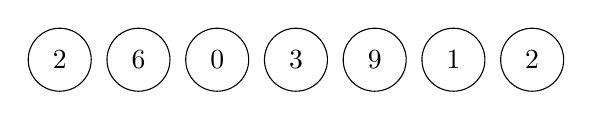
\begin{tikzpicture}
    \foreach \x/\n in {1/2, 2/6, 3/0, 4/3, 5/9, 6/1, 7/2} {
      \draw (\x, 0) circle (0.4) node {\n};
    }
  \end{tikzpicture}
  \caption{
    An instance of a seven coin game on a uniform distribution of
    $\{ 0, 1, \hdots, 9\}$. The first player has a strategy that allows her to
    win by one point.
  }
\end{figure}

\begin{question}
  For some fixed $\omega$, what is
  the expected first player's score of Peter Winkler's Coins-in-a-Row game when
  played with $X_1(\omega), X_2(\omega), \hdots, X_3(\omega)$ where both players
  are using a min-max strategy?
\end{question}

\begin{note}
  Let \[
    e = E[X_2 + X_4 + \hdots + X_{2n}] \text{ and }
    o = E[X_1 + X_2 + \hdots + X_{2n - 1}]
  \]
  When played with $2n$ coins, the first player's score is bounded below by $
    \max(e, o) - \min(e, o)
  $ by the strategy outlined by Peter Winkler.

  Trivially the first player's score is bounded above by the expected value of
  the $n$ largest coins minus the expected value of the $n$ smallest coins.
\end{note}

\begin{related}
  \item If all possible $n$-coin games are played with coins marked $0$ and $1$,
    how many games exist where both players have a strategy to tie.
  \item How does this change when played according to the (fair) Thue-Morse sequence?
  \item What if the players are cooperating to help the first player make as
    much as possible (with perfect logic)?
  \item What is both players are using the greedy algorithm?
  \item What if one player uses the greedy algorithm and the other uses min-max?
    (i.e. What is the expected value of the score improvement when using the
    min-max strategy?)
  \item What if one player selects a coin uniformly at random, and the other
    player uses one of the above strategies?
\end{related}
\end{document}
